%\documentclass[english,twoside]{article}
\documentclass[english,twoside]{labmanual} 
%labmanual.cls is a modified version of article.cls, tweaked to handle \part{} differently

%% LyX 1.1 created some parts of this file.  For more info, see http://www.lyx.org/.
%% Do not edit unless you really know what you are doing.

\usepackage[T1]{fontenc}
\usepackage[nomarginpar]{geometry}
\usepackage{tocloft} %Allow us to leave page numbers for Parts out of table of contents
\cftpagenumbersoff{part} %No page numbers for Parts out of table of contents
\renewcommand{\cftsecdotsep}{\cftsubsecdotsep}
%\usepackage{newclude} %Allows use of /include*{}
%DANGER DANGER: newclude is NOT compatible with package xr, used for external references.
\geometry{verbose,letterpaper}
\usepackage{fancyhdr}
\usepackage{babel}
\setlength\parskip{\medskipamount}
\setlength\parindent{0pt}
\usepackage{graphicx}
\usepackage{wrapfig}
%\usepackage{epstopdf} %this package apparently allows pdflatex to work on this document, since all we use are eps figures.
\usepackage{comment}
\usepackage{esvect}
\usepackage{amsmath} %uncommented by MT 5/2015, used in "E near charged rod"
\usepackage{mathtools} %added by MT 6/2015, for access to dcases environment in finding_v_from_e
\usepackage{tabularx} %added by MT 6/2015, for fixed width columns, used in rc_circuits
\usepackage{microtype}
\usepackage{titlesec}
\usepackage{xr}

%For fixed width columns:
\newcolumntype{L}[1]{>{\raggedright\arraybackslash}p{#1}}
\newcolumntype{C}[1]{>{\centering\arraybackslash}p{#1}}
\newcolumntype{R}[1]{>{\raggedleft\arraybackslash}p{#1}}


\addtolength{\oddsidemargin}{1.0cm} %without these two lines, larger margin is on the OUTSIDE.  We want the larger edge on the INSIDE, to allow room for the three hole punches
\addtolength{\evensidemargin}{-1.0cm}

\setlength\topmargin{0.2in}
\addtolength{\hoffset}{-1.0cm}
\addtolength{\textwidth}{2.0cm}
\addtolength{\voffset}{-1.5cm} %This line is apparently needed on some versions of MikTex XeLatex.  Comment out if your pages appear shifted too high.
\addtolength{\textheight}{3.5cm}
% define a strut for extra vertical space in tables.
\newcommand{\hi}{\rule[-2mm]{0mm}{6mm}}

\pagestyle{fancy}
%\fancyhead[LE,RO]{\slshape \rightmark} %This is the default for fancy page style
%\fancyhead[LO,RE]{\slshape \leftmark}
\fancyhead[LO,RE]{\slshape \rightmark} 
\fancyhead[LE,RO]{\slshape \leftmark} % Reversed LE, RO to  LO,RE to make headers come out correctly on even/odd pages



%%%%%%%%%%%%%%%%%%%%%%%%%%%%%% LyX specific LaTeX commands.
\providecommand{\LyX}{L\kern-.1667em\lower.25em\hbox{Y}\kern-.125emX\@}
\newenvironment{LyXParagraphIndent}[1]%
{
  \begin{list}{}{%
    \setlength\topsep{0pt}%
    \addtolength{\leftmargin}{#1}
    \setlength\parsep{0pt plus 1pt}%
  }
  \item[]
}
{\end{list}}
%% Special footnote code from the package 'stblftnt.sty'
%% Author: Robin Fairbairns -- Last revised Dec 13 1996
\makeatletter
\let\SF@@footnote\footnote
\def\footnote{\ifx\protect\@typeset@protect
    \expandafter\SF@@footnote
  \else
    \expandafter\SF@gobble@opt
  \fi
}
\expandafter\def\csname SF@gobble@opt \endcsname{\@ifnextchar[%]
  \SF@gobble@twobracket
  \@gobble
}
\edef\SF@gobble@opt{\noexpand\protect
  \expandafter\noexpand\csname SF@gobble@opt \endcsname}
\def\SF@gobble@twobracket[#1]#2{}
\makeatother


%I make use of some latex features to manage the section numbers. To use those you have to insert the following lines into the latex preamble (before the %"\begin{document}" command).

% two new commands to do labelling. - gpg 12/4/13
\newcommand{\customlabel}[2]{%
\protected@write \@auxout {}{\string \newlabel {#1}{{#2}{}}}}

\newcommand{\actlabel}[1]{%
\protected@write \@auxout {}{\string \newlabel {#1}{{\arabic{activity}}{}}}}

\newcommand{\makelabheader}
%{Name: \rule{2.0in}{0.1pt}\hfill{}Section: \rule{1.0in}{0.1pt}\hfill{}Date: \rule{1.0in}{0.1pt}}
{Name: \rule{2.0in}{0.1pt}\hfill{}Lab Partner(s): \rule{3.0in}{0.1pt}}

%\newcommand{\dir131}{../../131/StudentGuideModule1} %This does not work, because commands can only be made of numeric characters, not numbers.

%A new command for putting a box around a paragraph:
\newenvironment{newboxed} %maybe there's a better way to do this.  I just cribbed from the web. --MT
    {\begin{center}
    \begin{tabular}{|p{0.9\textwidth}|}
    \hline\\
    }
    { 
    \\\\\hline
    \end{tabular} 
    \end{center}
    }

\newcounter{activity}

%  The following command, \answerspace, should be used to replace \vspace.
%  \vspace{} is not ideal for an answer space for students, for two reasons:
%  1. It can be ignored if it comes at the end of a page, and
%  2. The spacing is exact, and Latex will not stretch or compress it at all to make things fit on a page, which means
%  that other things WILL get stretched or compressed to make things fit, which means those other things will 
%  end up looking bad, and leading to a lot of underfull \vbox warnings.
%  \answerspace fixes both of those problems, specifically allowing the space to grow to up to twice the stated size.
\newcommand{\answerspace}[1]{\vspace*{#1 plus #1}}

%  The next several lines implement \includelab, which replaces \include.
%  Usage is \includelab{1}{file} to include it, or \includelab{0}{file} to NOT include it.  
%  But all 0's can be overridden by writing \includealllabstrue in the master.tex file, which is easier than deleting 
%  fifty individual `%' signs and then remembering to put them all back, which is what you had to do before.
%  \includeonly still works as you expect it to.
\newif\ifincludealllabs
\newcommand{\includelab}[2]{
	\ifnum#1=1
		\include{#2}
	\else {
		\ifincludealllabs
		 	\include{#2}
		\fi}
	\fi
}
 %all general latex packages, commands, and definitions now here.
\externaldocument{master}

%syntax: \includeonly{lab1,lab2,lab3} with no spaces after the commas.
%\includeonly{biot_savart_law/biot_savart_law, charge_density/charge_density,eoverm/eoverm }
%DANGER: The includeonly statement will make a document that does NOT have sequential page numbers.

\newcommand{\supplementmark}{HN}

\titleformat{\section}{\normalfont\Large\bfseries}{\supplementmark \thesection}{1em}{}
\fancyhead[LO,RE]{\slshape \rightmark} 
\fancyhead[LE,RO]{\slshape \supplementmark \leftmark} % Reversed LE, RO to  LO,RE to make headers come out correctly on even/odd 

\begin{document}

\setcounter{page}{165}  %Set this to desired first page
\setcounter{section}{38} %set this to desired first section number MINUS ONE

%--------------------------------------------
%Put include statements for labs below here.

\section{The Electrical and Gravitational Forces\footnote{
1990-93 Dept. of Physics and Astronomy, Dickinson College. Supported by FIPSE
(U.S. Dept. of Ed.) and NSF. Portions of this material have been modified locally
and may not have been classroom tested at Dickinson College.
} }

\makelabheader %(Space for student name, etc., defined in master.tex)

\begin{quote}
I began to think of gravity extending to the orb of the moon, and . . . I deduced
that the forces which keep the planets in their orbs must be reciprocally as
the squares of their distances from the centers about which they revolve: and
thereby compared the force requisite to keep the moon in her orb with the force
of gravity at the surface of the earth, and found them to answer pretty nearly.
All this was in the two plague years of 1665 and 1666, for in those days I was
in the prime of my age for invention, and minded mathematics and philosophy
more than at any time since. - Isaac Newton 
\end{quote}
\textbf{Objective }

To understand the similarities of the gravitational and electrical forces. 

\textbf{Overview }

The enterprise of physics is concerned ultimately with mathematically describing
the fundamental forces of nature. Nature offers us several fundamental forces,
which include a strong force that holds the nuclei of atoms together, a weak
force that helps us describe certain kinds of radioactive decay in the nucleus,
the force of gravity, and the electromagnetic force. 

\textit{Two kinds of force dominate our everyday reality-the gravitational force
acting between masses and the Coulomb force acting between electrical charges.}
The gravitational force allows us to describe mathematically how objects near
the surface of the earth are attracted toward the earth and how the moon revolves
around the earth and planets revolve around the sun. The genius of Newton was
to realize that objects as diverse as falling apples and revolving planets are
both moving under the action of the same gravitational force. 

\answerspace{0.3cm}
\begin{center}
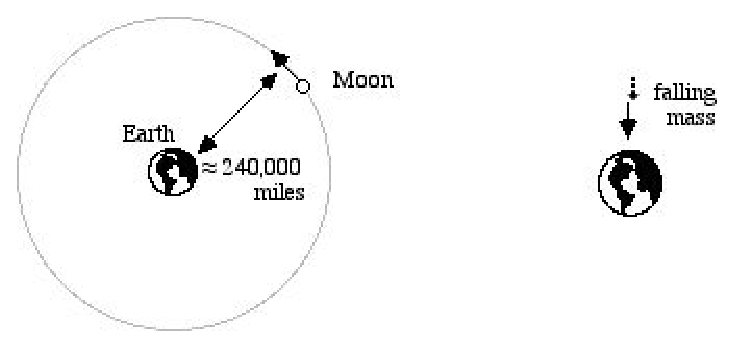
\includegraphics[width=0.9\textwidth]{elec_grav/elec_grav_fig1.eps} 
\end{center}
\answerspace{0.3cm}


\pagebreak[2]
Similarly, the Coulomb force allows us to describe how one charge \char`\"{}falls\char`\"{}
toward another or how an electron orbits a proton in a hydrogen atom. 

\answerspace{0.3cm}
\begin{center}
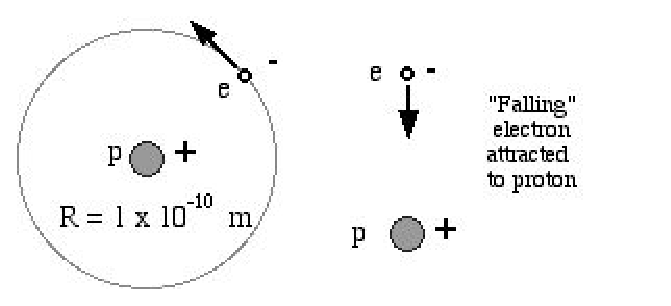
\includegraphics[width=0.9\textwidth]{elec_grav/elec_grav_fig2.eps} 
\end{center}
\answerspace{0.3cm}

The fact that both the Coulomb and the gravitational forces lead to objects
falling and to objects orbiting around each other suggests that these forces
might have the same mathematical form. 

In this unit we will explore the mathematical symmetry between electrical and
gravitational forces for two reasons. First, it is beautiful to behold the unity
that nature offers us as we use the same type of mathematics to predict the
motion of planets and galaxies, the falling of objects, the flow of electrons
in circuits, and the nature of the hydrogen atom and of other chemical elements.
Second, what you have already learned about the influence of the gravitational
force on a mass can be applied to aid your understanding of the forces on charged
particles. 

\textbf{Activity 1: Comparison of Electrical and Gravitational Forces }

Let's start our discussion of this comparison with the familiar expression of
the Coulomb force exerted on charge 1 by charge 2. 

\answerspace{0.3cm}
{\par\centering 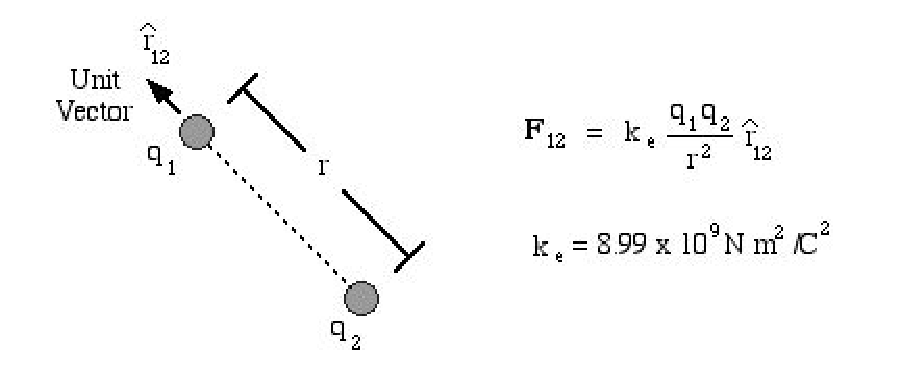
\includegraphics{elec_grav/elec_grav_fig3.eps} \par}
\answerspace{0.3cm}

Charles Coulomb did his experimental investigations of this force in the 18th
century by exploring the forces between two small charged spheres. Much later,
in the 20th century, Coulomb's law enabled scientists to design cyclotrons and
other types of accelerators for moving charged particles in circular orbits
at high speeds. 

Newton's discovery of the universal law of gravitation came the other way around.
He thought about orbits first. This was back in the 17th century, long before
Coulomb began his studies. A statement of Newton's universal law of gravitation
describing the force experienced by mass 1 due to the presence of mass 2 is
shown below in modern mathematical notation: 

\vspace{0.3cm}
{\par\centering 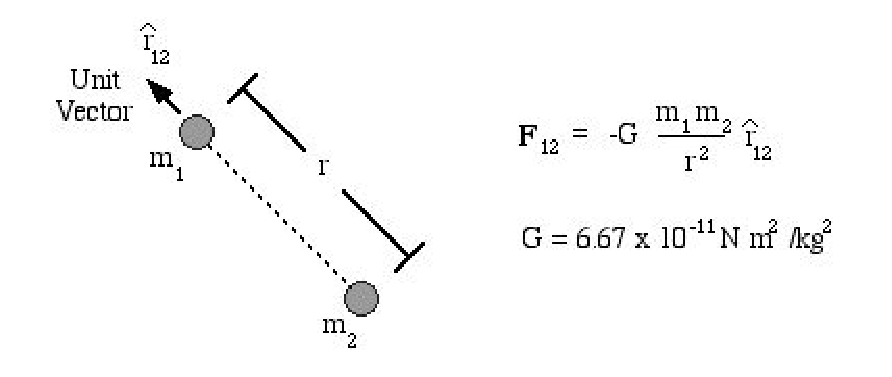
\includegraphics{elec_grav/elec_grav_fig4.eps} \par}
\vspace{0.3cm}

About the time that Coulomb did his experiments with electrical charges in the
18th century, one of his contemporaries, Henry Cavendish, did a direct experiment
to determine the nature of the gravitational force between two spherical masses
in a laboratory. This confirmed Newton's gravitational force law and allowed
him to determine the gravitational constant, G. A fact emerges that is quite
amazing. Both types of forces, electrical and gravitational, are very similar.
Essentially the same mathematics can be used to describe orbital and linear
motions due to either electrical or gravitational interactions of the tiniest
fundamental particles or the largest galaxies. This statement needs to be qualified
a bit when electrons, protons and other fundamental particles are considered.
A new field called quantum mechanics was developed in the early part of this
century to take into account the wave nature of matter, which we don't actually
study in introductory physics. However, even in wave mechanical calculations
electrical forces like those shown above are used. 

\textbf{Activity 2: The Electrical vs. the Gravitational Force} 

Examine the mathematical expression for the two force laws.

(a) What is the same about the two force laws?
\answerspace{20mm}

(b) What is different? For example, is the force between two like masses attractive
or repulsive? How about two like charges? What part of each equation determines
whether the like charges or masses are attractive or repulsive?
\answerspace{20mm}

(c) Do you think negative mass could exist? If there is negative mass, would
two negative masses attract or repel?
\answerspace{20mm}

\textbf{Which Force is Stronger-- Electrical or Gravitational?} 

Gravitational forces hold the planets in our solar system in orbit and account
for the motions of matter in galaxies. Electrical forces serve to hold atoms
and molecules together. If we consider two of the most common fundamental particles,
the electron and the proton, how do their electrical and gravitational forces
compare with each other?

Let's peek into the hydrogen atom and compare the gravitational force on the
electron due to interaction of its mass with that of the proton to the electrical
force between the two particles as a result of their charge. In order to do
the calculation you'll need to use some well known constants.

Electron: m\( _{e} \) = 9.1 x 10\( ^{-31} \) kg, q\( _{e} \) = - 1.6 x 10\( ^{-19} \)
C 

Proton: m\( _{p} \) = 1.7 x 10\( ^{-27} \) kg, q\( _{p} \) = +1.6 x 10\( ^{-19} \)
C 

Distance between the electron and proton: r = 0.53 x 10\( ^{-10} \) m

\textbf{Activity 3: The Electrical vs. the Gravitational Force in the Hydrogen
Atom}

(a) Calculate the magnitude of the electrical force on the electron. Is it attractive
or repulsive?
\answerspace{20mm}

(b) Calculate the magnitude of the gravitational force on the electron. Is it
attractive or repulsive?
\answerspace{20mm}

(c) Which is larger? By what factor (i.e. what is the ratio)?
\answerspace{20mm}

(d) Which force are you more aware of on a daily basis? If your answer does
not agree with the result of part (c), explain why, i.e. why do we usually not 
experience electrical forces in our everyday lives?
\answerspace{20mm}

\textbf{Activity 4: The Gravitational Force of the Earth}

(a) Use Newton's law to show that the magnitude of the acceleration due to gravity
on an object of mass m at a height h above the surface of the earth is given by
the following expression:
\[
\frac{GM_{e}}{\left( R_{e}+h\right) ^{2}}\]

Hint: Because of the spherical symmetry of the Earth you can treat the mass
of the Earth as if it were all concentrated at a point at the Earth's center.
\answerspace{20mm}
\pagebreak

(b) Calculate the acceleration due to gravity of a mass m at the surface of
the earth (h=0). The radius of the earth is R\( _{e} \) \( \approx  \) 6.38
x 10\( ^{3} \) km and its mass M\( _{e} \) \( \approx  \) 5.98 x 10\( ^{24} \)
kg. Does the result look familiar? How is this acceleration related to the gravitational
acceleration g?
\vspace{40mm}

(c) Use the equation you derived in part (a) to calculate the acceleration due
to gravity at the ceiling of the room you are now in. How does it differ from
the value at the floor? Can you measure the difference in the lab using the
devices available?
\vspace{30mm}

(d) Suppose you travel halfway to the moon. What is the new value of the acceleration due to gravity (neglecting the effect of the moon's pull)? (Recall that the earth-moon distance is about 384,000 km.)
\vspace{30mm}

(e) Is the gravitational acceleration \char`\"{}constant\char`\"{}, g, really
a constant? Explain.
\vspace{30mm}

(f) In part (d) you showed that there is a significant gravitational attraction
halfway between the earth and the moon. Why, then, do astronauts experience
``weightlessness'' when they are orbiting a mere 120 km above the earth?



\section{The Electric Field and the Electric Potential I}

\makelabheader %(Space for student name, etc., defined in master.tex)

\textbf{Objective}

\begin{itemize}
\item To investigate the electric field and potential of a point charge.
\end{itemize}

\textbf{Apparatus}

\begin{itemize}
\item Electric field and potential simulation entitled {\it EMField}.
\end{itemize}

\textbf{Introduction}

The direction of an electric field is the direction of the force on
a tiny positive test charge placed in the region of space where the
field is to be measured. If the magnitude of this test charge is infinitesimally
small, so small that it will not displace or disturb the charges that
are the source of the field, we can use the test charge to determine
quantitatively the strength of the electric field. The strength of
the electric field is taken to be the electric force, $F$, on the test
charge divided by the magnitude of the test charge, \( q_{t} \):
\( E=\frac{F}{q_{t}} \). The force (Coulomb's Law) between two charges,
\( q_{1} \) and \( q_{2} \), is \( F=k\frac{q_{1}q_{2}}{r^{2}} \),
where \( k \)= 9 x 10\( ^{9} \) Nm\( ^{2} \)/C\( ^{2} \). The units
of \( E \) are newtons per coulomb, so another way of describing the field
strength is to say it is the force experienced by a unit positive
test charge.

Recall from a previous laboratory exercise that the potential difference
between two points A and B, V\( _{B} \) - V\( _{A} \), is the work
done carrying a unit positive charge from point A to point B. Also,
the lines of force (the electric field lines) are always perpendicular
to the equipotential lines, lines on which all points are at the same
potential. In a static electric field, the electric potential difference
between two points is a constant and does not depend on the path used
for its computation. The absolute potential, as opposed to the potential
difference, is the amount of work done in carrying a unit charge from
infinity to point B. The magnitude of the absolute potential, then,
is computed as the integral from infinity to the point B of the electric
field.

\textbf{Investigation 1: A Single Charge}

\textbf{Activity 1: The Electric Field}

(a) (Note: you will need to run the program \filename{EMField} on a ``virtual machine''; see Appendix \ref{virtual_machine}.)  Go to \filename{Start $\rightarrow$ Programs $\rightarrow$ Physics Applications} and open the program \filename{EMField}. 
Click on the screen and you will see a screen with a set of
instructions.
Go to the \textbf{Sources} menu and select \textbf{3D Point Charges}.
A blank `table top' with a set of menu 
buttons at the top and bottom will appear. See Figure 1 below.

\begin{figure}[hbt]
\begin{center}
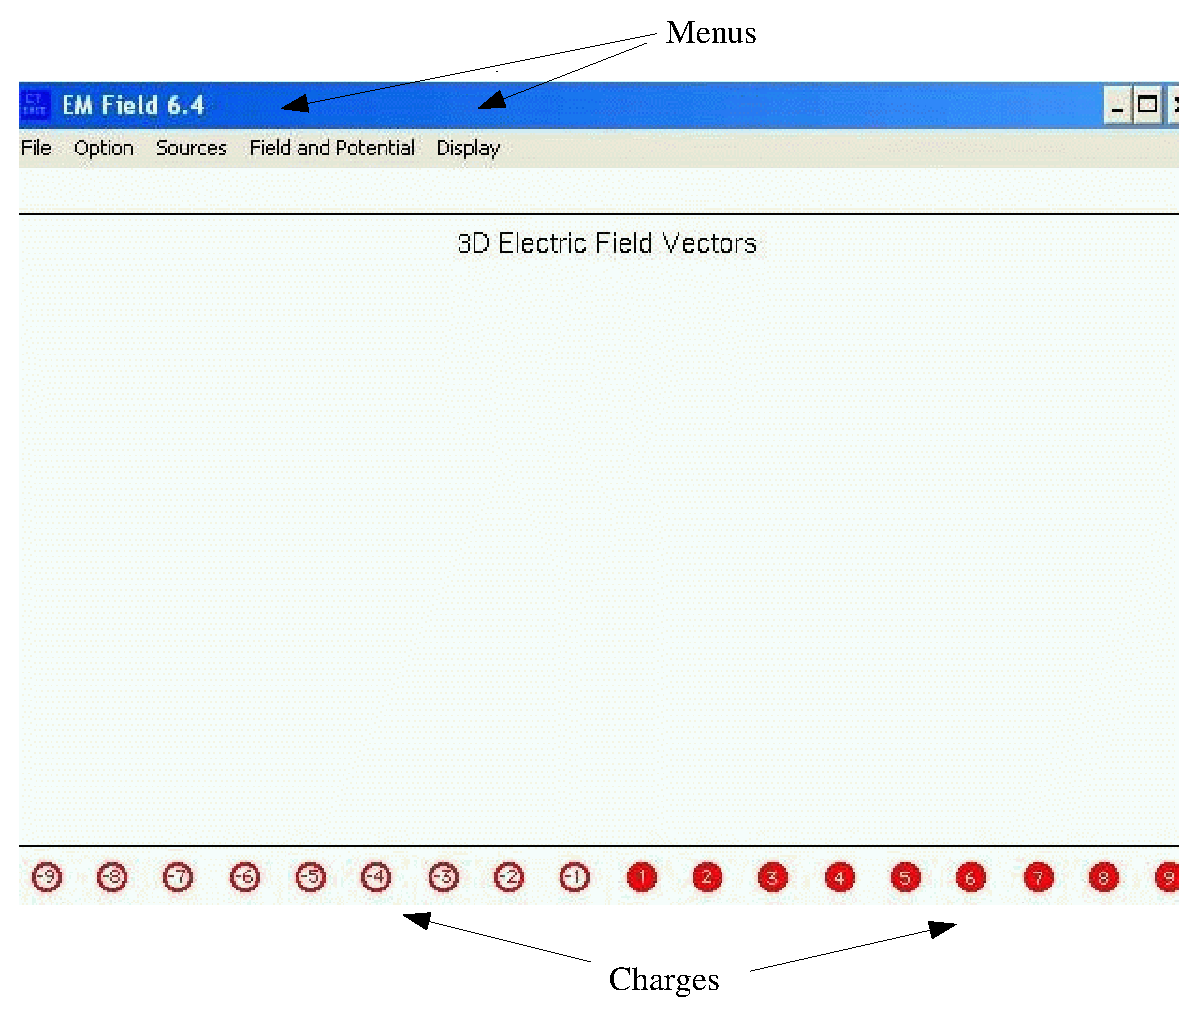
\includegraphics[height=4.0in]{electric_field_and_electric_potential/emfield1c.eps}
\caption{Table top for {\it EMField.}}
\index{color page}
\end{center}
\end{figure}

(b) Go to the {\bf Display} menu and set {\it EMField} to
{\bf Show Grid} and {\bf Constrain to Grid}.
These choices will make the following investigation a bit easier to perform.

(c) Select
the charge labeled {}``+4'' from the available set by clicking
on it and dragging it to the center of the table top. 

(d) \textbf{Prediction}: You will take measurements of the field at different
distances from the charge. You know the relative size of the
charge (+4), but you don't know the size of the charge in coulombs.
Generate an expression for the magnitude of the field from an unknown charge
with appropriate numerical constants and units.
The only unknown in your result should be the charge in coulombs.
How does the electric field depend on $r$, the distance from the point charge?
%\vspace{15mm}
\newpage

(e) Click anywhere in the table top and you will see an arrow drawn.
The size and direction of the arrow represent the magnitude and direction of
the electric field at that point due to the `+4' charge.
In what direction does the arrow point?
Click on the opposite side of the table top.
In what direction does this arrow point? How is it related to the first arrow?
\vspace{15mm}

(f) Click on many points so that you get a wide range of magnitudes from large
(barely fits on the table top) to small (barely bigger than a dot).

(g) Print the table top and use a ruler to measure the distance of each field 
point from the charge and the lengths of each of the arrows on your plot. 
Enter these data in the table below. Use the scale at the bottom of the table 
top to convert the length of each arrow into an electric field magnitude.
The units of the scale electric field vector are $1.0 ~ N/C$.

\vspace{0.3cm}
{\centering \begin{tabular}{|c|c|c|c|}
\hline 
~~~Distance from Charge (cm)~~~&
~~~Arrow Length (cm)~~~&
~~~Measured E (N/C)~~~\\
\hline
\hline 
&
&
\\
\hline 
&
&
\\
\hline 
&
&
\\
\hline 
&
&
\\
\hline 
&
&
\\
\hline 
&
&
\\
\hline 
&
&
\\
\hline 
&
&
\\
\hline 
&
&
\\
\hline
\end{tabular}\par}
\vspace{0.3cm}

%(h) Use the results in column 3 of your table to determine the unknown charge for each electric field measurement and enter the results in the table. NOTE: 
%For this calculation, assume the Coulomb's Law constant $k = 1.00 Nm^{2}/C^{2}$.
%This makes the charge a factor of about $10^{10}$ bigger than it is supposed to 
%be, but we are focussing here on how the electric field varies with distance 
%from the charge. Calculate the average and standard deviation of the values 
%of the charge. Are your results consistent? Explain.
%\vspace{30mm}

(h) \textbf{Prediction}: From Coulomb's Law, we expect the spatial variation
of the field strength to obey a power law: \( \left| E\right| =Ar^{n} \),
where \( A \) and \( n \) are constants. What do you predict the value of 
\( n \) to be?\vspace{15mm}

(i) Graph field strength as a function of $r$. Using the power fitting
function, determine the power of the function, $n$, and record it here.
Attach the plot to this unit.
\vspace{15mm}

(j) Does your result agree with your prediction? Explain any discrepancy.
\vspace{15mm}

\vspace{0.5in}
\textbf{Activity 2: The Electric Potential}

(a) Under the {\bf Display} menu click on {\bf Clean up Screen} to erase the
electric field vectors.

(b) \textbf{Prediction}: You will now take measurements of the potential.
How do you expect the electric potential to change with distance from the point
charge?
\vspace{15mm}
 
(c) Click on the \textbf{Potential} option under the \textbf{Field and Potential} menu. Click on the table top and a marker will be
placed at that point and labeled with the value of the potential there.
Click on many spots on the table top from very close to the point charge to
far away.
When you are finished print the table top.
\vspace{5mm}

(d) Measure and record in the following table the values of the distance from the point charge and the potential.

\vspace{0.3cm}
{\centering \begin{tabular}{|c|c|}
\hline 
~~~Distance (cm)~~~&
~~~Measured V (volts)~~~\\
\hline
\hline 
&
\\
\hline 
&
\\
\hline 
&
\\
\hline 
&
\\
\hline 
&
\\
\hline 
&
\\
\hline 
&
\\
\hline 
&
\\
\hline 
&
\\
\hline
\end{tabular}\par}
\vspace{0.3cm}


%(e) Calculate the value of the electric potential at each of these points
%from the distance you measured from the point charge and the value of the 
%charge from the previous activity. Again, assume $k = 1.00 Nm^{2}/C^{2}$.
%Fill in the appropriate columns of the table  with the distance
%and predicted potential. Show a sample calculation in the space below.
%\vspace{1in}


%(f) Did the measured values agree with your calculations? If they didn't,
%can you explain why not?\vspace{25mm}

(e) \textbf{Prediction}: From Coulomb's Law and the definition of the
electric potential, we expect the spatial variation of the potential
to obey a power law: \( \Delta V=Br^{m} \), where \( B \) and \( m \)
are constants. What do you predict the value of \( m \) to be?
\vspace{12mm}

(f) Graph the voltage as a function of $r$. Using the power fitting
function, determine the power of the function, $m$, and record it here.
\vspace{12mm}

(g) Does your result agree with your prediction? Explain any discrepancy.
\vspace{12mm}

\textbf{Activity 3: Field Lines and Equipotentials}

(a) Under the {\bf Display} menu click on {\bf Clean up Screen} to erase the 
potential values.

(b) Click on {\bf Field Lines} under the {\bf Field and Potential} menu. Click on many spots on the table top all around the charge to create field lines. Why are they straight lines?
\vspace{30mm}

(c) Click on {\bf Directional Arrows} under the {\bf Field and Potential} menu. Click on many spots to create directional arrows for the field lines. (Remember, electric field is a vector quantity.) Why are they directed away from the charge?
\vspace{30mm}

(d) Click on {\bf Equipotentials} under the {\bf Field and Potential} menu. Click on many spots to create equipotential lines. Why are they all circular?
\vspace{30mm}

(e) What is the relationship between the field lines and the equipotentials at 
the points where they cross?

%
\section{The Electric Field and the Electric Potential II}

\makelabheader %(Space for student name, etc., defined in master.tex)

\textbf{Objective}

\begin{itemize}
\item To investigate the electric field and potential of a charge distribution.
\end{itemize}

\textbf{Apparatus}

\begin{itemize}
\item Electric field and potential simulation entitled {\it EMField}.
\end{itemize}

\textbf{Introduction}

In the previous unit (which we will refer to as Investigation 1) we studied the dependence
of the electric field and the electric potential on $r$, the distance from a
single charge.
Now we will study the same ideas for a different charge distribution.

\textbf{Investigation 2: Four Symmetrically Arranged Charges}

\textbf{Activity 1: The Electric Field}

(a) Go to \filename{Start $\rightarrow$ Programs $\rightarrow$ Physics Applications} and open the program \filename{EMField}.
(Or, if it's already running, use the options under the 
\textbf{Display} menu to clear the table top and delete any charges.)
Go to the \textbf{Sources} menu and select \textbf{3D Point Charges}.
A blank `table top' with a set of menu 
buttons at the top and bottom will appear (see Figure 1 in Investigation 1, the previous unit).

(b) Go to the \textbf{Display} menu and set {\it EMField} to
{\bf Show Grid} and {\bf Constrain to Grid} if they are not already set.
These choices will make the following investigation a bit easier to perform.

(c) Under \textbf{Sources}, click on \textbf{3D Point Charges}. Select the
charge labeled {}``+4'' from the available set by clicking on it.
Add four individual charges, arranging them symmetrically within about
1 cm of the central point where the {}``+4'' charge was located
in Investigation 1 (the previous unit). 

(d) {\bf Prediction:} How will the electric field be oriented within the region of the four charges?
How will the field be oriented outside the region of the four charges?
How will the field depend on $r$, the distance from the center of the four charges, at large $r$?
\answerspace{25mm}

(e) Click anywhere in the table top and you will see an arrow drawn.
The size and direction of the arrow represent the magnitude and direction of
the electric field at that point due to the four charges.
In what direction does the arrow point?
Click on the opposite side of the table top.
In what direction does this arrow point? How is it related to the first arrow?
\answerspace{15mm}

(f) Click on many points so that you get a wide range of magnitudes from large
(barely fits on the table top) to small (barely bigger than a dot).

\pagebreak[2]
(g) Print the table top and use a ruler to measure the lengths of each of the arrows on your plot, for points \textbf{outside} the region of the four charges. Enter this data in the following table. Use the scale at the bottom of the table top to convert the length of each arrow into an electric field magnitude.
The units of the scale electric field vector are $1.0 ~ N/C$.

\vspace{0.3cm}
{\centering \begin{tabular}{|c|c|c|}
\hline 
~~~Distance from Charge Center (cm)~~~&
~~~Arrow Length (cm)~~~&
~~~Measured E (N/C)~~~\\
\hline
\hline 
&
&
\\
\hline 
&
&
\\
\hline 
&
&
\\
\hline 
&
&
\\
\hline 
&
&
\\
\hline 
&
&
\\
\hline 
&
&
\\
\hline 
&
&
\\
\hline 
&
&
\\
\hline
\end{tabular}\par}
\vspace{0.3cm}


(h) \textbf{Prediction}: From Coulomb's Law, we expect the spatial variation
of the field strength to obey a power law: \( \left| E\right| =Ar^{n} \),
where \( A \) and \( n \) are constants. What do you predict the
value of \( n \) to be?
\answerspace{15mm}

(i) Graph your results. Using the power fitting
function, determine the power of the function, $n$, and record it here.
Attach the plot to this unit.
\answerspace{15mm}

(j) Does your result agree with your prediction? Explain any discrepancy.\vspace{15mm}

\textbf{Activity 2: The Electric Potential}

(a) Under the {\bf Display} menu click on {\bf Clean up Screen} to erase the
electric field vectors.

(b) \textbf{Prediction}: You will now take measurements of the potential.
How do you expect the electric potential to change with distance from the center of the four charges?
\answerspace{15mm}
 
(c) Click on the \textbf{Potential} option under the \textbf{Field and Potential} menu. Click on the table top and a marker will be
placed at that point and labeled with the value of the potential there.
Click on many spots on the table top from very close to the charges to
far away.
When you are finished print the table top.
\answerspace{15mm}

\pagebreak
(d) Measure and record in the following table the values of the distance from the center of the point charge region (for points outside the region of the four charges) and the potential.

\vspace{0.3cm}
{\centering \begin{tabular}{|c|c|c|}
\hline 
~~~Distance from Charge Center (cm)~~~&
~~~Measured V (volts)~~~\\
\hline
\hline 
&
\\
\hline 
&
\\
\hline 
&
\\
\hline 
&
\\
\hline 
&
\\
\hline 
&
\\
\hline 
&
\\
\hline 
&
\\
\hline 
&
\\
\hline
\end{tabular}\par}
\vspace{0.3cm}


(e) \textbf{Prediction}: From Coulomb's Law and the definition of the
electric potential, we expect the spatial variation of the potential
to obey a power law: \( \Delta V=Br^{m} \), where \( B \)
and \( m \) are constants. What do you predict the value of \textbf{\( m \)}
to be?\vspace{20mm}


(f) Graph your results. Using the power fitting
function, determine the power of the function, $m$, and record it here.
\vspace{20mm}

(g) Does your result agree with your prediction? Explain any discrepancy.\vspace{20mm}

(h) How do your results for the power constants, $n$ and $m$, of the four
symmetrically-arranged charges compare with the power constants you
determined in Investigation 1 (the previous unit) for the single point charge?\vspace{20mm}

(i) What can you conclude about the field and potential effects due to
a distribution of charge outside the region of the distribution (in
relation to a single point charge)?



\section{The Electric Field and the Electric Potential III}

\makelabheader %(Space for student name, etc., defined in master.tex)

\textbf{Objective}

\begin{itemize}
\item To investigate the electric field and potential of an electric dipole.
\end{itemize}

\textbf{Apparatus}

\begin{itemize}
\item Electric field and potential simulation entitled {\it EMField}.
\end{itemize}

\textbf{Introduction}

In the previous units (which we will refer to as Investigation 1 and 2) we studied the dependence
of the electric field and the electric potential on $r$, the distance from
a charge distribution.
Now we will study the same ideas for a charge distribution commonly found in physics and chemistry
using the same methods we used before.

\textbf{Investigation 3: An Electric Dipole}

\textbf{Activity 1: The Electric Field}

(a) Start the program \filename{EMField} (under \filename{Start $\rightarrow$ Programs $\rightarrow$ Physics Applications}) or use the options under the 
\textbf{Display} menu to clear the table top and delete any charges.
Go to the \textbf{Sources} menu and select \textbf{3D Point Charges}.
A blank `table top' with a set of menu 
buttons at the top and bottom will appear.

(b) Go to the {\bf Display} menu and set {\it EMField} to
{\bf Show Grid} and {\bf Constrain to Grid} if they are not already set.
These choices will make the following investigation a bit easier to perform.

(c) Clear the table top and build an electric dipole by placing two magnitude
{}``8'' charges of opposite sign a distance 4 cm apart near the lower left 
of the table top, oriented along a horizontal line. Put the positive charge 
on the left.


(d) {\bf Prediction} How will the electric field be oriented between the two charges? How will the field be oriented outside the region of the two charges?
How will the field depend on $r$, the distance from the midpoint of a line joining the two charges, at large $r$?
\vspace{25mm}

(e) Click along a line \textit{perpendicular to the midpoint of a line joining the two charges}. The size and direction of the arrow represent the magnitude and direction of the electric field at that point due to the dipole.
In what direction does the arrow point?
\vspace{15mm}

(f) Click on many points along the same line so that you get a wide range of 
magnitudes from large (barely fits on the table top) to small (barely bigger 
than a dot).

(g) Print the table top and use a ruler to measure the lengths of each of the 
arrows on your plot and the distance from the midpoint of a line joining the 
two charges. Enter these data in the following table. Use the scale at the 
bottom of the table top to convert the length of each arrow into an electric 
field magnitude. The units of the scale electric field vector are $1.0 ~ N/C$.

\vspace{0.3cm}
{\centering \begin{tabular}{|c|c|c|}
\hline 
~~~Distance from Charge Center (cm)~~~&
~~~Arrow Length (cm)~~~&
~~~Measured E (N/C)~~~\\
\hline
\hline 
&
&
\\
\hline 
&
&
\\
\hline 
&
&
\\
\hline 
&
&
\\
\hline 
&
&
\\
\hline 
&
&
\\
\hline 
&
&
\\
\hline 
&
&
\\
\hline 
&
&
\\
\hline
\end{tabular}\par}
\vspace{0.3cm}


(h) \textbf{Prediction}: From Coulomb's Law, we expect the spatial variation
of the field strength to obey a power law: \( \left| E\right| =Ar^{n} \),
where \( A \) and \( n \) are constants. What do you predict the
value of \( n \) to be?\vspace{15mm}

(i) Graph your results. Using the power fitting
function, determine the power of the function, $n$, and record it here.
Attach the plot to this unit.
\vspace{15mm}

(j) Does your result agree with your prediction? Explain any discrepancy.\vspace{15mm}

(k) How do your results compare with the power law constants you found
in Investigations 1 and 2? Explain.\vspace{15mm}


\textbf{Activity 2: The Electric Potential}

(a) Under the {\bf Display} menu click on {\bf Clean up Screen} to erase the
electric field vectors.

(b) Reverse the two charges, i.e. put the positive charge on the right, keeping 
the same distance between the charges.

(c) \textbf{Prediction}: You will now take measurements of the potential.
How do you expect the electric potential to change with distance from the 
electric dipole \textit{along the axis of the dipole} (the line joining 
the two charges defines the axis)?
\vspace{15mm}
 
(d) Click on the \textbf{Potential} option under the \textbf{Field and Potential} menu. Click on the table top and a marker will be
placed at that point and labeled with the value of the potential there.
Click on many spots on the table top along the axis of the dipole (outside the dipole itself). When you are finished print the table top.
\vspace{15mm}

(e) Measure and record in the following table the values of the distance from 
the midpoint of a line joining the two charges and the potential.

\vspace{0.3cm}
{\centering \begin{tabular}{|c|c|c|}
\hline 
~~~Distance from Charge Center (cm)~~~&
~~~Measured \( \Delta  \)V (volts)~~~\\
\hline
\hline 
&
\\
\hline 
&
\\
\hline 
&
\\
\hline 
&
\\
\hline 
&
\\
\hline 
&
\\
\hline 
&
\\
\hline 
&
\\
\hline 
&
\\
\hline
\end{tabular}\par}
\vspace{0.3cm}


(f) \textbf{Prediction}: From Coulomb's Law and the definition of the
electric potential, we expect the spatial variation of the potential
to obey a power law: \( \Delta V=Br^{m} \), where \( B \)
and \( m \) are constants. What do you predict the value of \textbf{\( m \)}
to be?\vspace{15mm}


(g) Graph your results. Using the power fitting
function, determine the power of the function, $m$, and record it here.
\vspace{15mm}

(h) Does your result agree with your prediction? Explain any discrepancy.
\vspace{15mm}

(i) How do your results compare with the power law constants you found
in Investigations 1 and 2? Explain.\vspace{15mm}


\textbf{Activity 3: Equipotential Lines and Field Lines}

(a) Under the \textbf{Display} menu click on \textbf{Clean up Screen} to erase the potential values.

(b) Under the \textbf{Field and Potential} menu, drag down to \textbf{Equipotentials}.
Click the mouse on the table top and a
line will be drawn representing the equipotential line with a label
representing the value of the electric potential. {[}If
the curve does not close (i.e., the last point drawn doesn't match
up with the starting point), consult the instructor.{]} Map out the
equipotential lines by moving the cursor across the table top away
from each charge and clicking the mouse at regular intervals.

(c) What do these curves represent?\vspace{15mm}

(d) Under the \textbf{Field and Potential} menu, click on \textbf{Field Lines}.
The field lines of the charge distribution will be drawn. {[}If \textit{EMField} takes a long time to draw one of the field lines, consult your instructor.{]}
Print the result and attach it to this unit.
 
(e) How are the field lines and the equipotential lines related to one
another at the points where they cross?




\section{Capacitance Series Circuit}

Name \rule{2.0in}{0.1pt}\hfill{}Section \rule{1.0in}{0.1pt}\hfill{}Date
\rule{1.0in}{0.1pt}

\textbf{Objective}

\begin{itemize}
\item To investigate the relationship among charge, potential difference, and capacitance in a series combination of capacitors.
\end{itemize}
\textbf{Introduction} 

In class the series combination of capacitors was studied with the assumption
of a constant potential difference energizing the circuit.  In practice this
is difficult to reproduce in the lab because capacitors typically do not
maintain a steady charge for very long.  To get around this we will energize
the circuit with an alternating potential difference provided by a sine wave
generator.  The relationships among $Q$, $V$, and $C$ are still the same, so
we can study these circuits in the lab.

For a series combination of capacitors, the total voltage across the circuit
is the sum of the voltages across the individual capacitors, that is

\begin{displaymath} V = V_1 + V_2 + V_3 \end{displaymath}

The equivalent capacitance of the combination is given by

\begin{displaymath} \frac{1}{C} = \frac{1}{C_1} + \frac{1}{C_2} + \frac{1}{C_3} \end{displaymath}

\textbf{Apparatus}

\begin{itemize}
\item Sine wave generator 
\item Capacitors of 1.0, 4.7, and 10 $\mu$f
\item Digital multimeter
\item Connecting leads
\end{itemize}
\textbf{Activity}

%\vspace{0.3cm}
%{\centering \resizebox*{0.45\textwidth}{!}{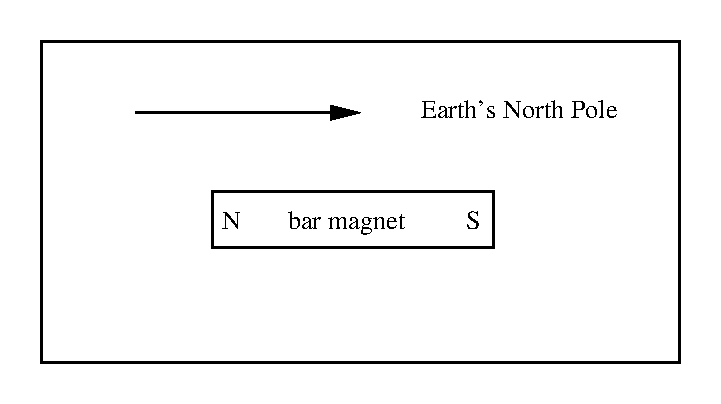
\includegraphics{magnetism_2_fig_1.eps}} \par}
%\vspace{0.3cm}

\begin{enumerate}
\item Connect the three capacitors in series with the sine wave generator.
\item Set the sine wave generator to 200 Hz (not critical) and adjust the
amplitude so that the output measures 5 to 6 volts as measured with the
digital multimeter set for \underline{AC volts}.
\item Using the multimeter, measure $V$ for the sine wave generator and also
for each of the individual capacitors (all with uncertainties) and
list them here. Don't forget units.\vspace{20mm}
\item Calculate the total voltage and its uncertainty from the first equation
above and compare with your measured value.  Do they agree?\vspace{30mm}
\item Assuming 10 percent uncertainties on each of the capacitances,
calculate the equivalent capacitance and its uncertainty from the second
equation above.\vspace{30mm}
\item Calculate the total charge for the circuit (and its uncertainty) from
$Q = CV$.\vspace{30mm}
\item \textbf{Prediction:} How will the charge on the individual capacitors
compare with the total charge calculated above?\vspace{30mm}
\item Calculate the charge on each capacitor (and its uncertainty) and compare with the total.
Do the results agree with your prediction?
\end{enumerate}


\section{Magnetism: Qualitative Interactions and Compasses}

\makelabheader %(Space for student name, etc., defined in master.tex)

\textbf{Objectives}

\begin{itemize}
\item To investigate the characteristics of magnets.
\item To understand how a compass works.
\end{itemize}
\textbf{Introduction} 

The electric interaction, you probably know, is not the only one in
which opposites attract and likes repel. Magnetic interactions have
similar characteristics. All simple magnets, regardless of size, are
bipolar: there are two magnetic poles. Consider this question, then:
Can we talk about like and unlike as we do for electricity?

\textbf{Apparatus}

\begin{itemize}
\item 2 bar magnets 
\item 2 cylindrical magnets 
\item rods and clamps
\item wool cloth
\item rubber rod
\item string
\end{itemize}
\textbf{Activity 1: The Characteristics of Magnets}

\begin{enumerate}
\item Feel the attraction between two magnets when pulled apart after having
come together without effort on your part. Describe qualitatively
in terms of strength and separation.\vspace{15mm}

\item Feel the repulsion when one of them is turned around and pushed toward
the other. Describe as in step 1.\vspace{15mm}

\item Note and describe the difference in (strength and direction of) interactions
between the ends and the middle.\vspace{15mm}

\end{enumerate}
\textbf{Activity 2: How a Compass Works}

\begin{enumerate}
\item Identify geographic north and south.
\item Hang one of the cylindrical magnets horizontally from a horizontal rod.
\item When it comes to rest, along which geographical line does the magnet
lie? \vspace{15mm}

\item Which end (colored or uncolored) is the \char`\"{}north-seeking\char`\"{}
end?\vspace{15mm}

\item Remove the cylindrical magnet and repeat step 2 with the second cylindrical magnet. Answer, again, the questions above.\vspace{15mm}

\item What happens when you bring the \char`\"{}north-seeking\char`\"{}
end of the first magnet near the hanging one's north-seeking end?\vspace{15mm}

\item What happens when you bring the first magnet's opposite end near the
second's north-seeking end?\vspace{15mm}

\item What about the first magnet's north-seeking end near the opposite
end of the hanging one?\vspace{15mm}

\item What happens when you bring the opposite ends near one another?\vspace{15mm}

\item Define in your own words like and unlike poles?\vspace{15mm}

\item What always happens between like poles?\vspace{15mm}

\item What always happens between unlike poles?\vspace{15mm}

\item Determine with a labelled bar magnet which end of your hanging magnet
should be identified as the north pole and which the south.
\vspace{10mm}
\item Why do we identify one end of a magnet as the north pole and the other
as the south?\vspace{15mm}

\item In your own words, explain a compass.\vspace{15mm}

\item In terms of magnetism, what is the earth?\vspace{15mm}

\item Charge a rubber rod with the wool cloth and bring it near the ends
of the suspended magnet; describe its effect on the magnet.\vspace{15mm}

\item Does a south magnetic pole repel a negative electric charge?\vspace{15mm}

\item Does a north magnetic pole attract a negative electric charge?\vspace{15mm}
\end{enumerate}



\section{Refraction of Light}

Name \rule{2.0in}{0.1pt}\hfill{}Section \rule{1.0in}{0.1pt}\hfill{}Date
\rule{1.0in}{0.1pt}

\textbf{Objective}

To investigate the path traveled by light through a plate of plexiglass
(a transparent solid material).

\textbf{Introduction}

The speed of light depends on the medium in which it travels. In passing
from one medium, at least some light energy is reflected. If the second
medium is transparent, most of the light will pass into and through
it. If the beam is not perpendicular to the boundary between the two
media, it will bend as it enters, an effect known as refraction. The
direction a single ray of light travels when refracted is given by
Snell's law:

\begin{displaymath} \frac{sin~i}{sin~r} = \frac{v_1}{v_2} = \frac{n_2}{n_1} \end{displaymath}

where

\begin{quote}
i = incident angle

r = refracted angle

v\( _{1} \) = light speed in medium 1

v\( _{2} \) = light speed in medium 1

n\( _{1} \) = index of refraction of medium 1 

n\( _{2} \) = index of refraction of medium 2
\end{quote}
\textbf{Note}: All angles are measured from the normal to the boundary
at the point the ray enters the medium. The index of refraction is
the ratio of light's speed in a vacuum, $c$, to its speed in the medium,
$v$: $n = c / v$. It is worth remembering that $n_{air} \approx 1.00$.

\vspace{0.3cm}
{\centering 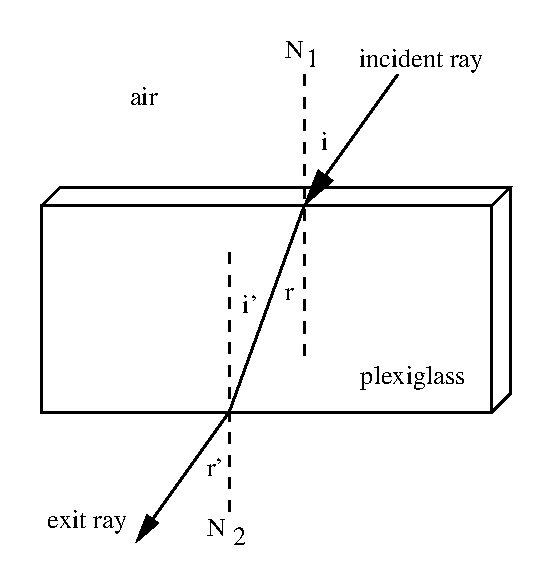
\includegraphics{refraction_of_light_fig_1.eps} \par}
\vspace{0.3cm}

\vspace{15mm}
\textbf{Apparatus} 

\begin{itemize}
\item light fence 
\item plexiglass block 
\item white paper, pins, and wood board 
\item protractor
\end{itemize}
\textbf{Activity} 

\begin{enumerate}
\item Put a plexiglass plate at the center of a piece of paper. Outline
its position. Identify a normal, $N_1$, perpendicular to an edge of
the plate.
\item Arrange the light source apparatus so that the parallel rays of light
cross the paper and are incident at a $30^\circ$-$35^\circ$ angle
to the normal. Trace one of these rays.
\item Sight the corresponding ray as it emerges from the other side of the
plexiglass. Trace this ray.
\item Construct the normal, $N_2$.
\item Measure and record $i$, $r$, $i'$, and $r'$. Compute and record $n_{plexiglass}$.\vspace{20mm}

\item Repeat the above procedure for different incident angles of between
$25^\circ$ and $40^\circ$.
\item Calculate and record an average $n_{plexiglass}$.\vspace{20mm}

\item Does $i = i'$? Explain.\vspace{15mm}

\item Does $r = r'$? Explain.\vspace{15mm}

\item Are the incident and exit rays parallel? Explain.\vspace{15mm}

\item What is the speed of light in the plexiglass?\vspace{15mm}

\item Under what conditions would a refraction angle be greater than an
incident angle?\vspace{15mm}
\end{enumerate}



\section{Refraction at Spherical Surfaces: Thin Lenses}

\makelabheader %(Space for student name, etc., defined in master.tex)

\textbf{Objective}

\begin{itemize}
\item To investigate thin lenses.
\end{itemize}
\textbf{Introduction} 

A lens converges or diverges light rays. It is a transparent material
bounded, in the case of thin lenses, by spherical edges. The line
between the centers of curvature of these edges is referred to as
the principal axis. The principal focus is the point on the principal
axis where parallel incident rays converge. The distance from the
lens to this point is known as the focal length. The relation between
the focal distance, $f$, the object distance, $p$, and the image distance,
$q$, is:

\begin{displaymath} \frac{1}{p} + \frac{1}{q} = \frac{1}{f}. \end{displaymath}

\textbf{Apparatus}

\begin{itemize}
\item light fence
\item converging (convex) lens in holder
\item converging and diverging lenses (1 each) without holders
\item optical bench 
\item light source with 12v output power source
\item optical viewing screen (white)
\item plastic ruler
\end{itemize}
%\textbf{Investigation 1: The Converging Lens}

\textbf{Activity 1}

\begin{itemize}
\item Arrange the light source apparatus so that the parallel rays of light
cross a piece of paper. 
\item Place a convex lens (without holder) on the paper perpendicular to the central ray.
Outline its position and the path of the rays. Pay particular attention
to the condition near the principal focus.
\item What is the focal length of this lens?\vspace{15mm}
\item Include a sketch of the light rays in your lab book, showing the focal point and focal length of the lens.
\end{itemize}
\textbf{Activity 2 }

\begin{itemize}
\item Place the light source in its bracket at one end of the optical bench. 
The arrow on the light source will be the object in this investigation. Measure
and record its height, $h_0$.\vspace{10mm}

\item Place a converging lens in its holder on the optical bench 70 cm from the object (this is the object distance $p$). Turn on the light source and position the optical viewing screen on the optical bench so that a sharp image of the arrow appears on the screen. Measure the distance of the screen from the lens. This is the image distance $q$. Also measure the height of the image $h_i$. Record $p$, $q$, and $h_i$ in the first line of the following table.
\end{itemize}
\vspace{0.3cm}
{\centering \begin{tabular}{|c|c|c|c|c|c|}
\hline 
~~~~~~~\( p \)~~~~~~~&
~~~~~~~\( q \)~~~~~~~&
~~~~~~~\( h_{i} \)~~~~~~~&
~~~~~~~\( \frac{h_{i}}{h_{0}} \)~~~~~~~&
~~~~~~~\( \frac{q}{p} \)~~~~~~~&
~~~~~~~\( f \)~~~~~~~\\
\hline
\hline 
&
&
&
&
&
\\
\hline 
&
&
&
&
&
\\
\hline 
&
&
&
&
&
\\
\hline 
&
&
&
&
&
\\
\hline 
&
&
&
&
&
\\
\hline
\end{tabular}\par}
\vspace{0.3cm}

\begin{itemize}
\item Move the lens to create four more object distances of 60, 50, 40, and 30 cm. In each case, measure the image distance and the height of the image and record in the above table. Calculate and record the ratios of the image and object heights, $h_i / h_0$, and the image and object distances, $q / p$. Record these values in the above table. You should now have the first five columns of the above table filled in.
\item Calculate and record the focal length, $f$, for each observation. Show one of the calculations here:\vspace{15mm}
\item Determine an average focal length, $f_{ave}$, and a standard
deviation based on your five values.\vspace{15mm}
\item What is the relationship between the ratio of the image to object
heights and the ratio of image and object distances? The first ratio
is called the magnification.\vspace{15mm}

\item Replace the converging lens with a diverging one. Try to obtain a
real image on the viewing screen.
\item Why can you not form a real image with a diverging lens?\vspace{15mm}

\end{itemize}
%\textbf{Investigation 2: Lenses in Combination (Optional)}

%\textbf{Activity}

%\begin{itemize}
%\item Place a converging lens and a diverging lens together into the lens
%holder. Check to see that you can get a real image with this combination.
%\end{itemize}
%\vspace{0.3cm}
%{\centering \begin{tabular}{|c|c|c|c|c|c|}
%\hline 
%~~~~~~~\( p \)~~~~~~~&
%~~~~~~~\( q \)~~~~~~~&
%~~~~~~~\( h_{i} \)~~~~~~~&
%~~~~~~~\( \frac{h_{i}}{h_{0}} \)~~~~~~~&
%~~~~~~~\( \frac{q}{p} \)~~~~~~~&
%~~~~~~~\( f \)~~~~~~~\\
%\hline
%\hline 
%&
%&
%&
%&
%&
%\\
%\hline 
%&
%&
%&
%&
%&
%\\
%\hline 
%&
%&
%&
%&
%&
%\\
%\hline 
%&
%&
%&
%&
%&
%\\
%\hline 
%&
%&
%&
%&
%&
%\\
%\hline
%\end{tabular}\par}
%\vspace{0.3cm}
%
%\begin{itemize}
%\item Repeat the five sets of observations of Investigation 1, Activity
%2, to get an equivalent focal length $f_{ave}^{eq}$.\vspace{40mm}
%
%\end{itemize}
%\textbf{Investigation 3: The Diverging Lens}
%
%\textbf{Activity 1 (Optional)}
%
%\begin{itemize}
%\item Using the relation:
%\end{itemize}
%\begin{displaymath} \frac{1}{f^{eq}} = \frac{1}{f_1} + \frac{1}{f_2}, \end{disp%laymath}
%
%\begin{quote}
%determine the focal length of the diverging lens, $f_2$. Use $f^{eq}_{ave}$
%for $f^{eq}$ and $f_{ave}$ for $f_1$.\vspace{2in}
%
%\end{quote}
\textbf{Activity 3}

\begin{itemize}
\item Repeat the procedure of Activity 1 with a concave
lens. Locate the principal focus by extending the refracted rays backwards.

\item What is the focal length of this lens?\vspace{15mm}
\item Include a sketch of the light rays in your lab book, showing the focal 
point and focal length of the lens.
\end{itemize}



\section{Charles' Law}

Name \rule{2.0in}{0.1pt}\hfill{}Section \rule{1.0in}{0.1pt}\hfill{}Date
\rule{1.0in}{0.1pt}+

\textbf{Objectives} 

To investigate the relationship between volume and temperature for
a constant mass of gas at constant pressure and determine the value
of absolute zero.

\textbf{Apparatus} 

\begin{itemize}
\item Charles law apparatus with stand.
\item Temperature sensor.
\item Air chamber, tubing, and ballast.
\item Containment vessel.
\end{itemize}
\vspace{0.3cm}

\begin{figure}[hbt]
\begin{center}
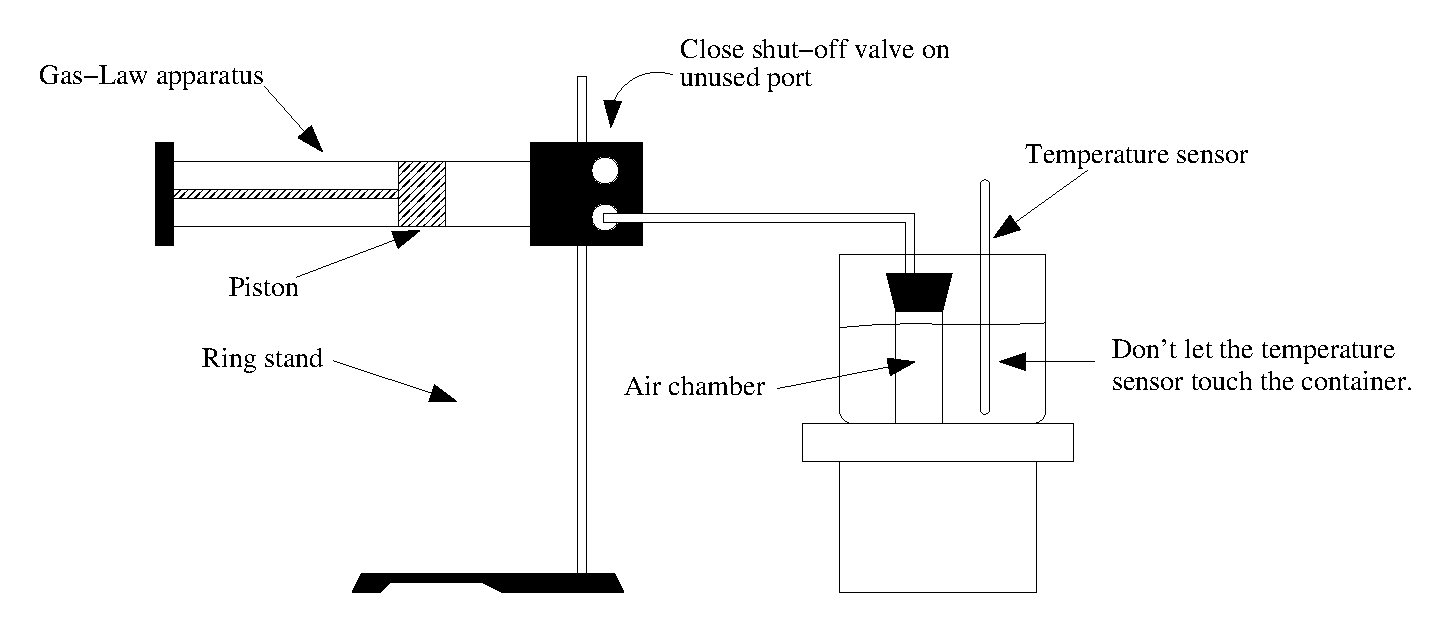
\includegraphics[width=6.0in]{charles_law_fig1.eps}
\caption{Charles' Law apparatus.}
\end{center}
\end{figure}

\textbf{Introduction}

The behavior of a gas can be described in terms of the macroscopic quantities:
temperature (T), pressure (P), and volume (V). The relationship between these
quantities is given by the equation of state of the gas. A real gas behaves
approximately as an ideal gas if it is far from liquefaction. In that case,
the equation of state of an ideal gas can be used to describe a real gas. For
a given mass of a gas, if one of the quantities P, T, or V is changed, a change
in the other two quantities probably will result. However, if one of the quantities
is kept constant, the relationship between the other two can be studied. The
relationship between temperature and volume of an ideal gas is called Charles' law.

The experimental apparatus is shown in the figure above and consists
of an air chamber containing dry air. The pressure on the air in the chamber is due to atmospheric
pressure applied through the movable piston.

\textbf{Activity 1: V-T Relationship for a Gas}

(a) Check that there are no leaks in the apparatus by trying to compressing
the piston from the 100 mm position to the 10 mm position. It should become
increasingly difficult to push the plunger as the volume decreases. If this
is not the case, check the couplings for fit. If no problem is obvious, then
consult your instructor. 

(b) Open the {\it Charles' Law} activity in the 132 Workshop Folder under the
{\bf Start} menu.
Click on the window labeled \textit{Charles' Law Table}. 
This is where your data will be displayed as you record
it. This table display will show the values of the gas temperature in the air chamber
and the entry number.
The data-taking procedure you will follow is described here first.
One member of your team will heat the air chamber in the flask on the hot plate 
and call out the position of the piston.
Another member will record the position settings by hand in the table below
and
click the {\bf Keep} button on the {\it DataStudio} interface to record the 
temperature for that entry.
To begin recording data, make sure the piston is at the low end of the scale, and click
the {\bf Start} button on the {\it DataStudio} interface. 
The {\bf Start} button will change to a {\bf Keep} button and the table
display will show the value of the temperature next to the first entry in the table. 
The reading in the temperature column should be colored red.
Click the {\bf Keep} button to record this temperature (notice the reading in the Temperature
column beside the entry number changes from red to black). The next entry number
 will appear in the Entry column of the data table display.

%NOTE: For the first temperature reading, the air in the chamber will be
%in thermal equilibrium with the environment. This will not be the case immediately
%after adding ice for the next reading. Therefore, you must allow
%3-5 seconds for the system to return to thermal equilibrium after you add ice
% and before clicking on {\bf Keep} to record temperature values. 

(c) Now, immerse the air chamber in a beaker of cold, tap water water and click
{\bf Start} on the {\it DataStudio} interface. You can monitor the temperature
on the temperature versus time plot to the right.
Make sure the set screw on the side of the piston is released.

(d) When the temperature is stable click {\bf Keep} and that point will be recorded in the
table. One team member should read off the piston position while the other 
writes it in the table at the same time.

(e) Now turn up the heat. The piston will move as the gas expands.
Read out the position of the piston every one or two millimeters. The other team member
will click {\bf Keep} (recording the temperature) and record the piston position
in the table.

(f) Repeat step (e) until the piston no longer moves or the water starts to boil.
 
(g) Calculate the volume of the apparatus for each piston position and plot
this volume versus temperature. The diameter of the Gas-Law apparatus is written on its
base.

\vspace{0.3cm}
{\centering \begin{tabular}{|c|c|c|c|}
\hline 
~~~Entry Number~~~&
~~~Piston Position (mm)~~~&
~~~Gas-Law Apparatus Volume (ml)~~~&
~~~Temperature ($^\circ  \rm C$)~~~\\
\hline
\hline 
&
&
&
\\
\hline 
&
&
&
\\
\hline 
&
&
&
\\
\hline 
&
&
&
\\
\hline 
&
&
&
\\
\hline 
&
&
&
\\
\hline 
&
&
&
\\
\hline 
&
&
&
\\
\hline 
&
&
&
\\
\hline
&
&
&
\\
\hline
&
&
&
\\
\hline
&
&
&
\\
\hline
&
&
&
\\
\hline
&
&
&
\\
\hline
\end{tabular}\par}
\vspace{0.3cm}

(h) How are the volume and temperature related?
Fit your data with the appropriate function and record the results here.
Print your plot and attach it to this unit.
\vspace{15mm}

(h) Repeat steps c-h to obtain a second {\it V-T} curve. Record your data in the table below
along with the fit to the V-T data.
\vspace{30mm}


\vspace{0.3cm}
{\centering \begin{tabular}{|c|c|c|c|}
\hline 
~~~Entry Number~~~&
~~~Piston Position (mm)~~~&
~~~Gas-Law Apparatus Volume (ml)~~~&
~~~Temperature ($^\circ  \rm C$)~~~\\
\hline
\hline 
&
&
&
\\
\hline 
&
&
&
\\
\hline 
&
&
&
\\
\hline 
&
&
&
\\
\hline 
&
&
&
\\
\hline 
&
&
&
\\
\hline 
&
&
&
\\
\hline 
&
&
&
\\
\hline 
&
&
&
\\
\hline
&
&
&
\\
\hline
&
&
&
\\
\hline
&
&
&
\\
\hline
&
&
&
\\
\hline
&
&
&
\\
\hline
\end{tabular}\par}
\vspace{2.0cm}

\textbf{Activity 2: Absolute Zero and the Kelvin Scale}

(a) The absolute zero of temperature can be defined as the temperature
at which the volume of an ideal gas is zero. Determine absolute
zero from the equations you obtained by fitting your V-T data.
\vspace{30mm}

(b) Determine the percent difference between your value of absolute
zero and the accepted value of -273\( ^{\circ } \)C. Are you happy or sad?
\vspace{30mm}

(c) Record the results from the other groups in class.
Obtain an average and standard deviation and record it here.
Are your results consistent with the class average? Explain.



%--------------------------------------------
\appendix
\setcounter{section}{4} %set this counter to number MINUS ONE corresponding to desired appendix letter. (4 for `E', etc.)
%Put include statements for supplementary appendices below here.
%                                                 
\section{Nuclear Safety}

All of the radioactive sources we will use in class are very low-level
isotopes referred to as ``license-free'' sources.
The following guidelines should be followed for handling radioactive
materials in the classroom.

%test comment by Matt
\begin{enumerate}

\item Eating, drinking, and application of cosmetics in the 
laboratory are not permitted.

\item Pipetting by mouth is never permitted. Use suction devices
such as pipette filters.

\item Gloves and lab coats should be worn when working with all liquid
isotopes.

\item Before leaving the lab, wash your hands thoroughly and check for
possible contamination with a survey instrument.

\item All radioactive liquid wastes are to be poured into the liquid
waste container, NEVER into a sink.

\item Report all spills, wounds, or other emergencies to your instructor.

\item Maintain good housekeeping at all times in the lab.

\item Store radioactive material only in the designated storage area. Do not
remove sources from the lab.

\end{enumerate}


\end{document}
